
% TODO: not relevant here, move to introduction
%Agricultural technologies have been a source of innovation since the dawn of humanity. The quest for more efficient food
%production has driven significant research, and above all, automation stands out as a paramount achievement in the
%modern world. A great tool to improve the automation process is \gls{IoT}, a concept that refers to the interconnection
%of physical devices in a diffused network; each device collects valuable and localized information that is used to
%improve efficiency, productivity, and decision making.\\

The goal of this chapter is to describe the the benefits and requirements for \gls{IoT} in agriculture and and to
describe some existing well-knwown solutions. In particular, we will give a brief introduction to the \gls{LoRaWAN}
protocol with a focus on some proposed use case scenarios.


\section{Benefits}
\label{sec: benefits}
The refinment of automation systems used in agriculture has been a costant interest throughout all history of
industry due to the huge positive impact it has brought to society. If \gls{IoT} is introduced
in agricultural contexts, it could bring lots of benefits:
\begin{itemize}
    \item Precision farming: IoT devices enable farmers to collect real-time data on environmental variables. This data
        helps optimize irrigation, fertilization, and pest control, leading to higher crop yields and reduced resource
        waste;
    \item Decision making: the generated data provides farmers with insights into crop health, growth
        patterns, and yield predictions. This allows them to make informed decisions regarding planting, harvesting, and
        resource allocation, resulting in better outcomes;
    \item Remote monitoring and management: farmers can remotely monitor their fields through IoT devices,
        reducing the need for constant physical presence. This is especially valuable for managing large or distant farms;
    \item Automation and labor savings: automation can handle tasks such as planting, irrigation, and
        harvesting. This not only reduces labor costs but also frees up farmers to focus on more strategic aspects of
        their operations;
    \item Knowledge sharing and collaboration: IoT platforms can facilitate the exchange of best practices, data, and
        insights among farmers, researchers, and agricultural experts, promoting knowledge sharing;
    \item Sustainability and environmental impact: trough optimized resource use, IoT contributes to more sustainable
        and environmentally friendly agricultural practices;
\end{itemize}

\section{Requirements}
Where \gls{IoT} is applied to agriculture, a set of unique and challenging requirements come into play:
\begin{itemize}
    \item Power management: many remote agricultural locations lack a reliable power source. Devices need to be
        designed with energy-efficient technology paired with high-energy batteries and/or alternative power sources like solar
        panels to ensure uninterrupted operation;
    \item Connectivity and coverage: many agricultural areas lack reliable internet connectivity, which can hinder
        transmissions between IoT devices and central systems. Even by using alternative solutions such as \glspl{LPWAN}
        like LoRaWAN or Bacco, long distances and physical barriers are problems that need to be faced;
    \item Reliability and fail-safeness: human operation is not always convenient or even possible in
        some cases, so having a fail-safe system is crucial to have maintain functionality;
    \item Physical damage: constant exposure to weather conditions undermines the integrity of the devices used in the
        open field, so it is important to use of materials that are resistant to such circumstances;
    \item Environmental impact: some ecosystems may be influenced by the introduction of alien objects or
        electromagnetic radiation;
    \item Cost: initial setup costs for devices, sensors, and infrastructure can be high, which may discourage small
        farmers from adopting these technologies;
    \item Regulations and compliance: different regions may have varying regulations concerning the elecromagnetic
        specturm usage, environmental monitoring, and technology deployment. Adhering to these regulations can be complex when
        implementing solutions across different areas;
    \item User-friendly interfaces: the user interfaces need to be intuitive, especially for farmers who might not
        have extensive technical knowledge.
\end{itemize}
This thesis will not comprehensively cover all the aspects mentioned above. Instead, it will just concentrate on the
communication protocol utilized by the network. While all efforts have been directed towards meeting the requirements,
it is important to note that mechanical, environmental, economic, and legal considerations will be left to future
discussions.

\section{An Already Available Technology: LoRaWAN}
One of the most promising technologies in \gls{IoT} for agrigulture is \gls{LoRaWAN}, an open protocol built on top of
Semtech's proprietary LoRa modulation. It provides all the necessary software components to build a suitable network
that is reliable, power efficient and scalable according to extensive past research. See \cite{lorawan_agriculture_1}
and \cite{lorawan_agriculture_2} for reference.\\
A LoRaWAN network consists of sender nodes and gateways. When a sender node broadcasts a LoRa transmission, it can be
received by one or more gateways, that can store the information or forward it to a web server through the Internet.
This kind of message is called uplink. Gateways might need to transmit data to the sender nodes, this kind message is
called downlink. Gateways can be self-owned with a custom configuration or can be part of an existing community such as
\gls{TTN} or Helium.\\
Senders can uplink at any time because gateways are always listening to transmissions. On the other hand, downlink
messages need to be scheduled as it is not always possible for a sender node to be listening continuously because of
the limited power budget. To achieve that, LoRaWAN defines 3 classes of devices called class A, class B and class C.
The classes are sorted by increasing energy demand, so class A stands out in agricultural
contexts thanks to its superior power efficiency when compared to classes B and C. In this mode, a downlink message can
only be sent in 2 time slots at pre-defined delays subsequently to the reception of an uplink message. Figure \ref{img:
lorawan class a} shows a schematic version of the time slot management.\\
Due to the precise time slot management, the LoRaWAN standard does not support repeaters. Successful research has been
done to overcome this limitation, see \cite{lorawan_range_extender}, however the additional required harware and the
lack of official support from the standard makes it unconvenient to use.

\begin{figure}[ht]
    \centering
    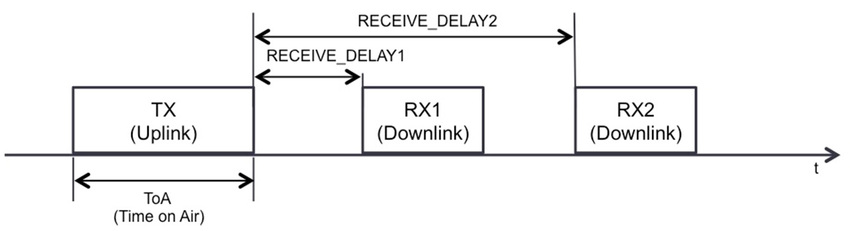
\includegraphics[width=\linewidth]{images/lorawan_class_a.png}
    \caption{LoRaWAN class A device operation.}
    \label{img: lorawan class a}
\end{figure}

\section{Real Word Use Case Scenario}
To better understand the limitations and the strenghts of LoRaWAN and Bacco, I will now describe 3 real world scenarios
in which \gls{IoT} can be integrated to achive the benefits described in Section \ref{sec: benefits}. All of them
require to collect physical data on a vineyard, however the locations and the surface areas are different for the 3
cases. Here follows a brief description of each of them:

\begin{enumerate}
    \item A small vineyard with an area of 1 hectar \footnote{1 hectar is equivalent to $10^4~\mathrm{m^2}$} which is
        located near an urban area and thus is fully covered by one or more hostpots registered on a public LoRaWAN
        network. The surface of the terrain is almost flat;
    \item A small vineyard with an area of 1 hectar which is located far from any urban area and thus is not fully
        covered by any public hostpot. The surface of the terrain is almost flat;
    \item A large vineyard with an area of 100 hectars which is located far from any urban area and thus is not covered
        by any public hostpot. The vineyard is spread across multiple hills.
\end{enumerate}

\subsection{LoRaWAN Setup Using A Public Gateway}
We will now analyze an \gls{IoT} network that makes use of a public infrastructure such as
\gls{TTN} or Helium. Each sender node can be easily registered on the platform and can transmit independently from the
other devices.\\
When trying to apply this solution to each of the described scenarios, we would observe the following behavior:
\begin{enumerate}
    \item Since the vineyard is covered by one or more public hotspots, it is possible to build the desired system.
        Depending to the distance from the hotspot, the sender nodes may be required to transmit at a high power in
        order for the signal to be detected by the hotspot. Any fault of nearby hotspots will result in an unusable and
        not directly fixable system;
    \item Since the vineyard is not fully covered by any public LoRaWAN network, it is not possible to build the desired
        system;
    \item Since the vineyard is not fully covered by any public LoRaWAN network, it is not possible to build the desired
        system.
\end{enumerate}
This is the simplest and cheapest proposed solution to implement, as no additional hardware is needed other than the
sender nodes, however it does not satisfy the requirements for 2 out of the 3 proposed scenarios.

\subsection{LoRaWAN Setup Using An Owned Gateway}
We will now analyze an \gls{IoT} network that makes use of owned/private LoRaWAN hotspots. Each
sender node can be connected to it and can transmit independently from the other devices.\\
When trying to apply this solution to each of the described scenarios, we would observe the following behavior:
\begin{enumerate}
    \item Since the vineyard is small and the underlying surface is mostly flat, the hotspot can fully cover it. The
        system will satisfy the requirements;
    \item Since the vineyard is small and the underlying surface is mostly flat, the hotspot can fully cover it. The
        system will satisfy the requirements;
    \item Since the vineyard is large and spread across multiple hills, it may not be possible for a single hotspot to
        cover the entirety of it because of physical barriers, so multiple hotspots would be needed to satify the
        requirements.
\end{enumerate}
The solution satisfies the requirements for all the scenarios, however in the $3^{rd}$ case it is necessary to use
multiple gateways to achieve full coverage. This makes the system very expencive and difficult to deploy.

\subsection{Bacco Setup}
Bacco is described in this thesis as an alternative to the discussed existing solutions. It has the goal to satisfy all
the requirements for the proposed scenarios and to provide a competitive system to LoRaWAN in the field of agriculture.
The next chapters will describe its implementation details and compare its performance to LoRaWAN's.
